\section{Реализация}
В этом разделе должны быть описаны средства, которые использовались при реализации системы, краткое описание программы. Исходный код можно посмотреть в репозитории \href{https://github.com/sanek701/SeaGame/tarball/master}{https://github.com/sanek701/SeaGame/tarball/master}.

Язык $Java$ обладает свойствами, необходимыми для удовлетворения требований системы:
		\begin{itemize}		
			\item Объектно-ориентированный;
			\item Объемная и простая в использовании библиотека для работы с графическими интерфейсами;
			\item Объемная и простая в использовании библиотека для работы с сетевыми соединениями;
			\item Многопоточность;
		\end{itemize}

Взаимодействие сервера и клиента реализовано путем сетевого соединения, то есть сервер может быть запущен на сторонней машине, к которой клиент просто будет присоединяться. Сервер может поддерживать одновременно несколько активных игр, что достигается при помощи параллельных потоков. Если у игрока неверные настройки, или сервер по какой-либо причине не работает, то игра не возможна. В случае активности несколько серверов можно подключиться к любому из них, изменив настройки соединения, а также у игрока есть возможность выбора игр, созданных другими пользователями. 
\begin{figure}[ht]
\centering
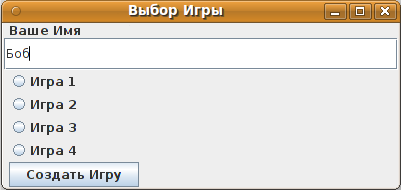
\includegraphics[width=10cm]{images/srn2.png}
\caption{Окно присоединения к игре}
\label{srn2}
\end{figure}

Основное окно клиента представляет собой размеченное поле, на котором проходит бой и небольшое текстовое поле для отображения системных сообщений. На рисунке [\ref{srn1}] представлено поле на начало боя, то есть когда все корабли уже расставлены, но ход никто не делал.

\begin{figure}[ht]
\centering
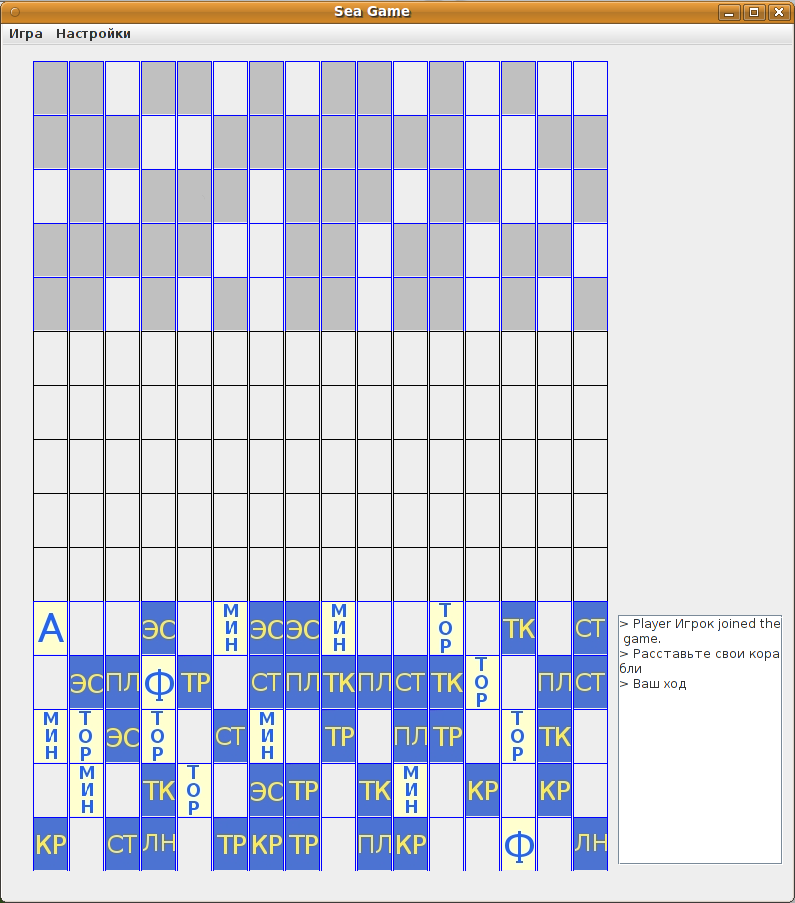
\includegraphics[width=15cm]{images/srn1.png}
\caption{Графический интерфейс}
\label{srn1}
\end{figure}



\endinput
